\begin{figure}[!t]
\centering
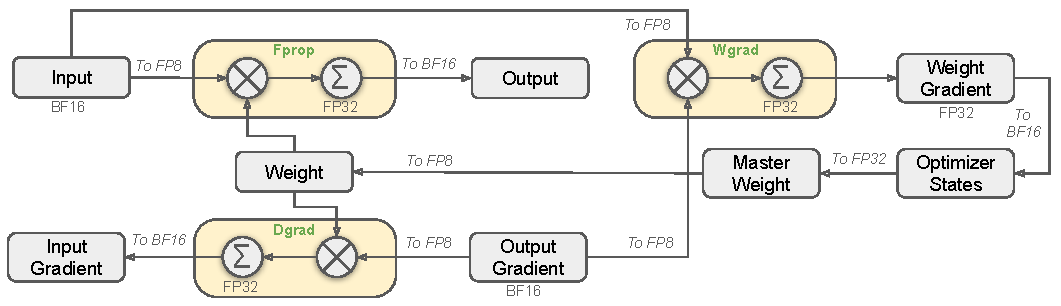
\includegraphics[width=0.99\linewidth]{figures/fp8-frameworkv3.pdf}
\caption{
    采用 FP8 数据格式的整体混合精度框架。为便于说明，图中仅展示 \texttt{Linear} 算子。
}
\label{fig:fp8_framework}
\end{figure}

受近期低精度训练进展的启发~\citep{fp8lm, llm.int8, 8-bit-numerical}，我们提出一种使用 FP8 数据格式训练 \dsviii{} 的细粒度混合精度框架。
尽管低精度训练很有前景，但它常受激活、权重和梯度中离群值的限制~\citep{massiveoutlier, understandoutlier, scalefp8train}。
虽然推理量化已取得显著进展~\citep{xiao2023smoothquant, frantar2022gptq}，但成功将低精度技术应用于大规模语言模型预训练的研究仍相对较少~\citep{scalefp8train}。
为应对这一挑战并有效扩展 FP8 格式的动态范围，我们引入一种细粒度量化策略：按包含 $1\times N_c$ 个元素的 tile 分组，或按包含 $N_c\times N_c$ 个元素的 block 分组。
在我们提高精度的累加过程中，相关的反量化开销得到大幅缓解，而这正是实现精确 FP8 General Matrix Multiplication~(GEMM) 的关键。
此外，为进一步降低 MoE 训练中的内存和通信开销，我们以 FP8 缓存和分发激活，同时以 BF16 存储低精度优化器状态。
我们在两个与 \dsvii{}-Lite 和 \dsvii{} 相近的模型规模上验证所提出的 FP8 混合精度框架，并训练约 1 万亿 token，更多细节见附录~\ref{app:fp8_cp_bf16}。
值得注意的是，与 BF16 基线相比，我们的 FP8-training 模型的相对损失误差始终低于 0.25\%，处于训练随机性可接受范围内。

\subsubsection{混合精度框架}
基于低精度训练中广泛采用的技术~\citep{bf16train, fp16train}，我们提出一个用于 FP8 训练的混合精度框架。
在该框架中，大多数计算密集型操作以 FP8 执行，而少数关键操作被有策略地保留为原始数据格式，以平衡训练效率与数值稳定性。
整体框架如图~\ref{fig:fp8_framework} 所示。

首先，为加速模型训练，大多数核心计算 kernel，即 GEMM 操作，都以 FP8 精度实现。
这些 GEMM 操作接受 FP8 张量作为输入，并输出 BF16 或 FP32。
如图~\ref{fig:fp8_framework} 所示，与 \texttt{Linear} 算子相关的三个 GEMM，即 \texttt{Fprop}，前向传播，\texttt{Dgrad}，激活反向传播，以及 \texttt{Wgrad}，权重反向传播，均以 FP8 执行。
相较原始 BF16 方法，该设计在理论上可使计算速度翻倍。
此外，FP8 \texttt{Wgrad} GEMM 允许以 FP8 存储激活，供反向传播使用。
这显著降低了内存消耗。

尽管 FP8 格式具有效率优势，某些算子由于对低精度计算敏感，仍需要更高精度。
此外，一些低成本算子也可以使用更高精度，而对整体训练成本只带来可忽略的开销。
因此，经过细致研究后，我们对以下组件保留原始精度，例如 BF16 或 FP32：embedding 模块、输出头、MoE gating 模块、归一化算子和注意力算子。
这些有针对性的高精度保留保证了 \dsviii{} 稳定的训练动态。
为进一步保证数值稳定性，我们以更高精度存储 master weights、权重梯度和优化器状态。
尽管这些高精度组件会带来一定内存开销，但在我们的分布式训练系统中，可通过跨多个 DP rank 的高效分片将其影响降至最低。

\begin{figure}[!t]
\centering
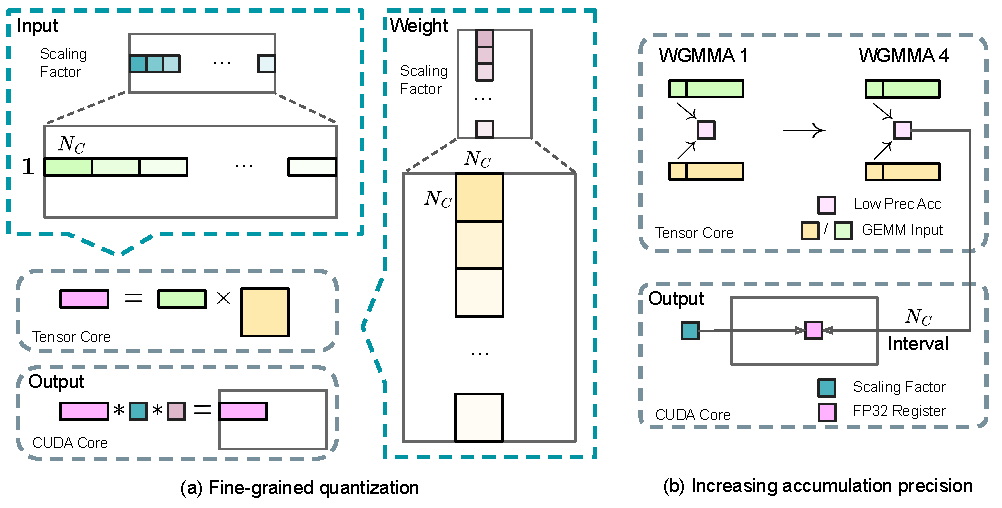
\includegraphics[width=0.95\linewidth]{figures/fp8-128accumulatorv4.pdf}
\caption{
    (a) 我们提出一种细粒度量化方法，以缓解特征离群值导致的量化误差；为简化说明，图中仅展示 \texttt{Fprop}。
    (b) 结合我们的量化策略，我们每隔 $N_C=128$ 个元素 MMA 将结果提升到 CUDA Cores 上进行高精度累加，从而提高 FP8 GEMM 精度。
}
\label{fig:fp8_quantization}
\end{figure}

\subsubsection{通过量化与乘法提升精度}
基于我们的混合精度 FP8 框架，我们引入若干策略来提高低精度训练精度，重点覆盖量化方法和乘法过程。

\paragraph{细粒度量化。}
在低精度训练框架中，由于 FP8 格式的动态范围有限，且受较少指数位约束，溢出和下溢是常见挑战。
标准做法是将输入张量的最大绝对值缩放到 FP8 的最大可表示值，从而使输入分布对齐到 FP8 格式的可表示范围~\citep{fp16train}。
这种方法使低精度训练对激活离群值高度敏感，从而严重降低量化精度。
为解决这一问题，我们提出一种细粒度量化方法，在更细粒度上应用缩放。
如图~\ref{fig:fp8_quantization} (a) 所示，(1) 对激活，我们按 \texttt{1x128} tile 对元素分组并缩放，即每个 token 每 128 个通道；(2) 对权重，我们按 \texttt{128x128} block 对元素分组并缩放，即每 128 个输入通道和每 128 个输出通道。
该方法使量化过程能够根据更小的元素组调整 scale，从而更好地适应离群值。
在附录~\ref{app:fp8_blockwise} 中，我们进一步讨论了像权重量化一样按 block 对激活分组和缩放时出现的训练不稳定性。

我们方法中的一项关键修改，是沿 GEMM 操作的内维引入 per-group 缩放因子。
标准 FP8 GEMM 并不直接支持这一功能。
不过，结合我们精确的 FP32 累加策略，它可以得到高效实现。
% We will elaborate it in the following paragraph.

值得注意的是，我们的细粒度量化策略与 microscaling formats 的思想高度一致~\citep{rouhani2023microscaling}，而 NVIDIA 下一代 GPU，Blackwell 系列，的 Tensor Cores 已宣布支持量化粒度更小的 microscaling formats~\citep{nvidia_tensor_cores}。
我们希望该设计能为后续工作提供参考，以跟上最新 GPU 架构的发展。

\paragraph{提高累加精度。}
低精度 GEMM 操作常遭遇下溢问题，其精度很大程度上依赖高精度累加，而高精度累加通常以 FP32 精度执行~\citep{bf16train, fp16train}。
然而，我们观察到 NVIDIA H800 GPU 上 FP8 GEMM 的累加精度仅能保留约 14 bit，显著低于 FP32 累加精度。
当内维 \texttt{K} 较大时，这一问题会更加突出~\citep{switchback}，而在扩大 batch size 和模型宽度的大规模模型训练中，这正是典型场景。
以 \texttt{K} = 4096 的两个随机矩阵 GEMM 操作为例，在我们的初步测试中，Tensor Cores 中有限的累加精度导致最大相对误差接近 2\%。
尽管存在这些问题，有限累加精度仍是一些 FP8 框架的默认选项~\citep{transformerengine}，严重限制了训练精度。

为解决这一问题，我们采用提升到 CUDA Cores 上进行更高精度计算的策略~\citep{Thakkar_CUTLASS_2023}。
该过程如图~\ref{fig:fp8_quantization} (b) 所示。
具体而言，在 Tensor Cores 上执行 MMA，Matrix Multiply-Accumulate，期间，中间结果以有限 bit 宽累加。
一旦达到 $N_C$ 的间隔，这些部分结果就会被复制到 CUDA Cores 上的 FP32 寄存器，并在那里执行全精度 FP32 累加。
如前所述，我们的细粒度量化沿内维 \texttt{K} 应用 per-group 缩放因子。
这些缩放因子可以在 CUDA Cores 上作为反量化过程高效相乘，只带来极小的额外计算成本。

值得注意的是，这一修改会降低单个 warpgroup 的 WGMMA，Warpgroup-level Matrix Multiply-Accumulate，指令发射率。然而，在 H800 架构上，两个 WGMMA 通常可以并发驻留：当一个 warpgroup 执行提升操作时，另一个可以执行 MMA 操作。该设计使两个操作能够重叠，从而保持 Tensor Cores 的高利用率。
基于我们的实验，将 $N_C=128$ 个元素，即 4 个 WGMMA，设为累加间隔，是在不引入显著开销的前提下明显提高精度的最小间隔。

\paragraph{尾数优先于指数。}
不同于以往工作采用的混合 FP8 格式 \citep{transformerengine, fp8lm, hfp8}，即在 \texttt{Fprop} 中使用 \texttt{E4M3}，4-bit 指数和 3-bit 尾数，在 \texttt{Dgrad} 和 \texttt{Wgrad} 中使用 \texttt{E5M2}，5-bit 指数和 2-bit 尾数，我们在所有张量上采用 \texttt{E4M3} 格式以获得更高精度。
我们认为该方法的可行性来自我们的细粒度量化策略，即 tile 和 block-wise 缩放。
通过在更小的元素组上操作，我们的方法在这些分组元素之间有效共享指数位，从而缓解有限动态范围的影响。

\paragraph{在线量化。}
Tensor-wise 量化框架~\citep{transformerengine, fp8lm} 采用延迟量化，它维护此前迭代中最大绝对值的历史记录，用以推断当前值。
为确保 scale 准确并简化框架，我们对每个 \texttt{1x128} 激活 tile 或 \texttt{128x128} 权重 block 在线计算最大绝对值。
基于该值，我们推导缩放因子，并将激活或权重在线量化为 FP8 格式。

\subsubsection{低精度存储与通信}
结合我们的 FP8 训练框架，我们通过将缓存激活和优化器状态压缩为更低精度格式，进一步降低内存消耗和通信开销。

\paragraph{低精度优化器状态。}
我们采用 BF16 数据格式而非 FP32 来跟踪 AdamW~\citep{adamW} 优化器中的一阶和二阶矩，且未观察到性能下降。
不过，master weights，由优化器存储，和梯度，用于 batch size 累积，仍保留为 FP32，以确保整个训练过程的数值稳定性。

\paragraph{低精度激活。}
如图~\ref{fig:fp8_framework} 所示，\texttt{Wgrad} 操作以 FP8 执行。
为降低内存消耗，自然的选择是以 FP8 格式缓存激活，供 \texttt{Linear} 算子的反向传播使用。
不过，为实现低成本高精度训练，我们对若干算子进行了特别处理：
\begin{quote}
\textbf{(1) 注意力算子之后的 \texttt{Linear} 输入。} 这些激活也会用于注意力算子的反向传播，因此对精度敏感。我们专门为这些激活采用定制的 \texttt{E5M6} 数据格式。此外，这些激活会在反向传播中从 \texttt{1x128} 量化 tile 转换为 \texttt{128x1} tile。为避免引入额外量化误差，所有缩放因子均采用 round scaled，即 2 的整数次幂。

\textbf{(2) MoE 中 SwiGLU 算子的输入。} 为进一步降低内存成本，我们缓存 SwiGLU 算子的输入，并在反向传播中重新计算其输出。这些激活也使用我们的细粒度量化方法以 FP8 存储，在内存效率与计算精度之间取得平衡。
\end{quote}

\paragraph{低精度通信。}
通信带宽是 MoE 模型训练中的关键瓶颈。
为缓解这一挑战，我们将 MoE up-projections 之前的激活量化为 FP8，然后应用 \texttt{dispatch} 组件，这与 MoE up-projections 中的 FP8 \texttt{Fprop} 兼容。与注意力算子之后的 \texttt{Linear} 输入类似，该激活的缩放因子为 2 的整数次幂。
类似策略也应用于 MoE down-projections 之前的激活梯度。
对于前向和反向的 \texttt{combine} 组件，我们均保留 BF16，以维持训练流水线关键部分的训练精度。
